\chapter{Podręcznik Użytkownika}
\label{ch:manual}

\section{Strona Domowa}

Po uruchomieniu aplikacji użytkownik zostaje przeniesiony na stronę domową. Znajdzie tam swoje notatki i zeszyty wraz z przyciskiem w prawym dolnym rogu służącym do tworzenia nowej notatki, jak również dodatkowe elementy w menu górnego paska, pozwalające na zmianę motywu, czy reset bazy danych w celu usunięcia wszystkich notatek. 

\begin{figure}[ht]
    \centering
    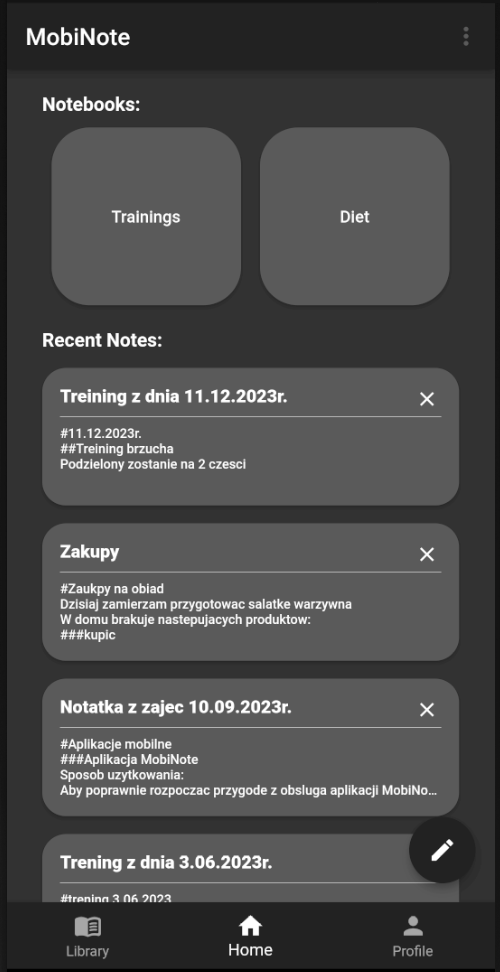
\includegraphics[height=10cm]{images/strona_domowa.png}
    \quad\quad
    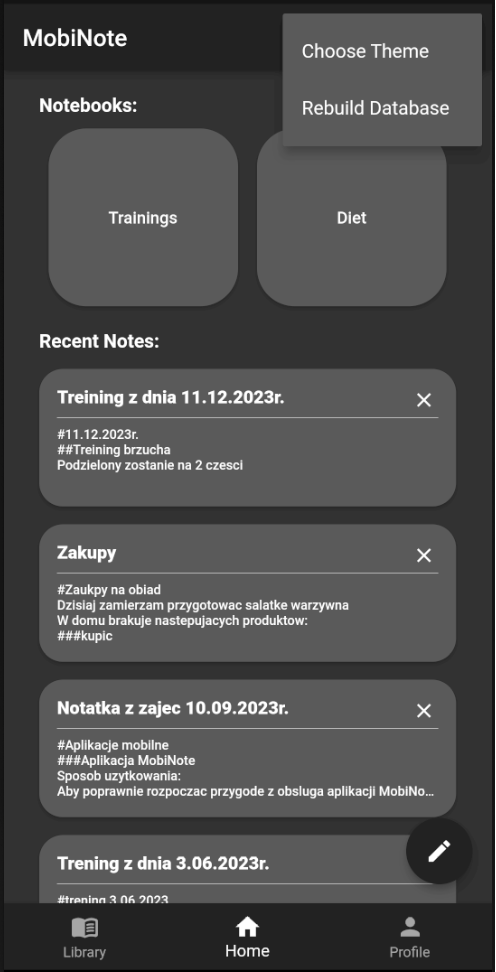
\includegraphics[height=10cm]{images/strona_domowa_opcje.png}
    \caption{Strona domowa aplikacji MobiNote z wybranym motywem \textbf{dark}.}
\end{figure}

\subsection{Opcja \textit{Choose Theme}}

Po uruchomieniu tej opcji wyświetli się okienko dialogowe z wyborem motywu, jakiego użytkownik chciałby użyć. Do wyboru mamy trzy mowtywy: \textbf{dark}, \textbf{light} oraz \textbf{easy}.

Motywy \textbf{dark} oraz \textbf{light} służą, jako główne motywy aplikacji, zachowując te same wielkości elementów tekstu i całej aplikacji.
Dla osób mających problemy z widocznością tekstu przy domyślnych ustawieniach wielkości i kolorów aplikacji przygotowany został mowtyw \textbf{easy}.
Motyw ten cechują kontrastujące ze sobą kolory, jak również zwiększone rozmiary czcionek, ikon, przycisków i paska narzędzi.

\begin{figure}[ht]
    \centering
    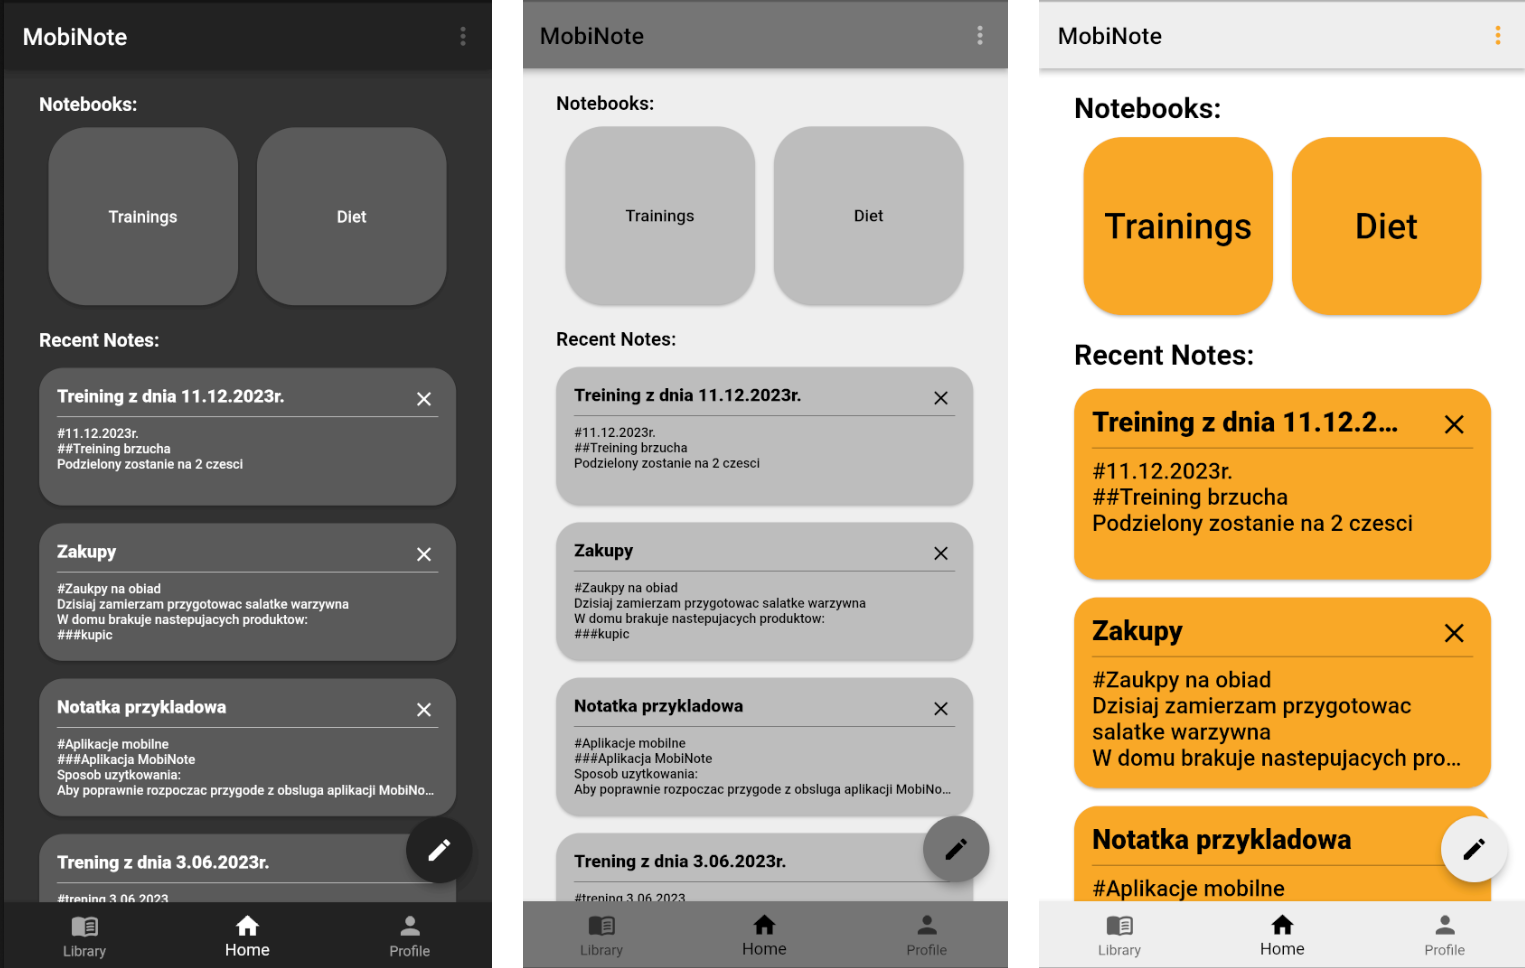
\includegraphics[height=8.5cm]{images/strona_domowa_motywy.png}
    \caption{Porównanie motywów na tej samej stronie domowej.}
\end{figure}

\subsection{Opcja \textit{Rebuild Database}}

Opcja ta otwiera okno dialogowe z pytaniem o to, czy na pewno chcemy wykonać tę przebudowanie bazy danych. Po zatwierdzeniu baza danych jest usuwana i budowana.

\subsection{Zeszyty}

Pod etykietą \textbf{\textit{Notebooks:}} widnieją dwa przyciski \textbf{Trainings} oraz \textbf{Diet}. Są to roboczo dodane przyciski, które są przygotowane pod rozszerzenie aplikacji w przyszłości o możliwość układania notatek w zeszyty, dla lepszej organizacji, a także wprowadzać etykiety.
Pomysł ten zostanie omówiony w rozdziale \textbf{Rozszerzenie Funkcjonalnosći aplikacji}.

\subsection{Notatki}

Kolejnym elementem strony domowej jest lista notatek znajdująca się pod etykietą \textbf{\textit{Recent Notes:}}. Każdy element zawiera tytuł oraz pierwsze cztery surowe linie tekstu(zawierające znaki specjalne styli w przypadku paragrafu będącego tekstem, lub string w formacie JSON reprezentujący widget zawarty w danym paragrafie).
W prawym górnym rogu elementów znajduje się przycisk \textbf{X} służący do usunięcia danej notatki z bazy danych.
Po naciśnięciu na dany element użytkownik zostaje przeniesiony do ekranu wyświetlania i edycji wybranej notatki.

W prawym dolnym rogu ekranu widnieje okrągły przycisk z ikoną ołówka.
Po jego naciśnięciu korzystający zostaje przeniesiony do ekranu edycji, gdzie może stworzyć i zapisać nową notatkę.

\section{Strona Edycji Notatki}

Po wybraniu notatki, lub przejściu do tworzenia nowej, na ekranie pojawi się strona edycji notatki. Składa się ona z głównego paska strony, paska narzędzi, oraz edytora.
\subsection{Pasek Strony}

\subsubsection{Przycisk Zapisu i Powrotu}

Aby wyjść i zapisać notatkę korzystający używa przycisku powrotu.
Ważnym jest, aby zamiast systemowych przycisków nawigacyjnych użyć właśnie tego przycisku nawigacyjnego, ponieważ wraz z powrotem do strony domowej zapisuje on notatkę, jeśli ta uległa zmianie.

Za zmianę notatki unawane są:

\begin{compactitem}
    \item edycja tekstu w paragrafie tekstowym
    \item edycja widgetu w paragrafie widgetu
\end{compactitem}
\vspace{5mm}

\textbf{WAŻNE!} Nowa notatka nie zostaje utworzona w momencie otwarcia okna edycji, a dopiero poprzez użycie przycisku powrotu pod warunkiem, ze jej tytuł lub zawartość uległy edycji. Oznacza to, że przejście do edycji nowej notatki, a następnie powrót, nie zapiszą pustej notatki, jednak dodanie i usunięcie znaku umożliwią zapis przy powrocie.

\subsubsection{Edytor tytułu}

Jest to pole tekstowe widniejące zaraz obok \textbf{Przycisku zapisu i powrotu}. Służy ono do edycji tytułu notatki.

\subsubsection{Przycisk zmiany opcji zapisu}

Ostatnim elementem paska jest \textbf{przycisk zmiany opcji zapisu}. Jest to przycisk typu \textbf{switch} domyślnie ustawiony na true. Każdorazowe kliknięcie zmienia jego logiczną wartość.
Wartość \textbf{true} oznacza zapis notatki w przypadku jej edycji, natomiast \textbf{false} oznacza brak zapisu stanu notatki, nawet jeśli została ona zmieniona.

\subsection{Pasek Narzędzi}

W tym pasku znajdują się przyciski oznaczone ikonami.
W aktualnej wersji aplikacji dostępne są dwa przyciski: dodanie obrazu(ikona obrazu), oraz dodanie listy(ikona listy).

\subsubsection{Dodanie obrazu}

Do zawartości notatki można dodawać również obrazy. Aby to zrobić należy kliknąć przycisk z ikoną obrazu na pasku narzędzi edytora notatki, a następnie wybrać z urządzenia zdjęcie, które ma zostać użyte. Zdjęcie zostanie dodane do notatki.

\subsubsection{Dodanie listy}

Po wybraniu tej opcji na ekranie pojawi się lista złożona początkowo z jednego elementu.
Jest on domyślnie ustwawiony na typ \textbf{checkbox}. Oznacza to, że jest to wiersz zawierający checkbox oraz puste pole tekstowe.

\subsection{Edytor Strony}

Edytor strony zajmuje reszę powierzchni ekranu. Jest polem, w którym następuje edycja tekstu oraz widgetów. Aktualny stan wizualny jest odświeżany na bieżąco, dzięki czemu użytkownik obserwuje zmiany jako efekt końcowy w czasie rzeczywistym.



\section{Edycja Zawartości Notatki}

\subsection{Paragrafy}

Notatki w aplikacji składają się z paragrafów, które dzielimy na paragrafy tekstowe i paragrafy widgetów.
Każdy paragraf może przechodzić w jedne z dostępnych trybów.
Obecnie wyróżnione są tryby:

\begin{compactitem}
    \item widoku
    \item edycji
    \item zaznaczenia
    \item niewidoczny
\end{compactitem}

\subsubsection{tryb widoku}

Paragraf istnieje w trybie widoku, kiedy nie jest aktywny.
Paragraf przechodzi w tryb widoku, w momencie przeniesienia aktywności na inny paragraf(na przykład poprzez kliknięcie).

\subsubsection{tryb edycji}

Paragraf przechodzi w tryb edycji, w momencie przeniesienia na niego aktywności.
Aktywność ta może zostać przeniesiona poprzez kliknięcie na elementy paragrafu, lub w przypadku, gdy jest to paragraf widgetów, a jego następnikiem jest paragraf tekstowy, którego edytujący stara się usunąć.

\subsubsection{tryb zanzaczenia}

Paragraf widgetów przechodzi w tryb zaznaczenia poprzez przytrzymanie jego elementów niebędących polem tekstowym(poniważ pole tekstowe ma już zarezerwowany ten gest na zaznaczanie tekstu).

\subsubsection{tryb niewidoczny}

Paragraf przestaje być widoczny w momencie przejścia edytora w kierunku pionowym wystarczająco do wysunięcia paragrafu poza edytor.

\pagebreak

\subsection{Edycja Paragrafów Tekstowych}

Każdy tekst zamykany jest w paragrafie tekstowym od początku, aż do znaku końca linii. Oznacza to, że styl, jaki zostanie nadany na początku linii zostanie zaaplikowany na całą linię. Przykładem jest ustawienie paragrafu jako nagłówka.

\subsubsection{Dodawanie}

Dodawanie paragrafów tekstowych odbywa się za pomocą klawiatury. W momencie, gdy użytkownik podczas edycji doda znak nowej linii, wówczas utworzy się nowy paragraf, będący następnikiem edytowanego.

\textbf{Ważne:} Podczas dodawania nowego paragrafu widgetów utworzy się nowy paragraf tekstowy jako jego następnik. Ma to na celu zachowanie możliwości ciągłej pracy z tekstem.

\subsubsection{Usuwanie}

Usunąć paragraf tekstowy można poprzez naciśnięcie przycisku \textbf{delete} na samym początku tekstu. Jeśli poprzedni paragraf jest paragrafem tekstowym, wówczas pozostały tekst kopiowany jest na koniec poprzedniego paragrafu.

\subsubsection{Ustawianie nagłówka}

Ustawienie nagłówka odbywa się poprzez wstawienie znaku \textbf{\#} na początku linii, przed tekstem.

\subsubsection{Dostępne nagłówki}
\begin{itemize}
    \setlength\itemsep{0mm}
    \item nagłówek1 \textbf{\#}
    \item nagłówek2 \textbf{\#\#}
    \item nagłówek3 \textbf{\#\#\#}
    \item nagłówek4 \textbf{\#\#\#\#}
\end{itemize}

Brak nagłówka oznacza, że dana linia jest zwykłym paragrafem o domyślnej wielkości czcionki i odstępów oraz nie zawiera pogrubienia.

\pagebreak

\subsubsection{Odkrywanie znaków nagłówka}

Edytor posiada funcję odkrywania znaków nagłówka, w celu ułatwienia edycji danego nagłówka. Dzięki temu użytkownik może zobaczyć który aktualnie nagłówek jest wybrany oraz w prosty sposób przechodzić pomiędzy typami nagłówków dodając bądź usuwając znak \textbf{\#}.


\begin{figure}[ht]
    \centering
    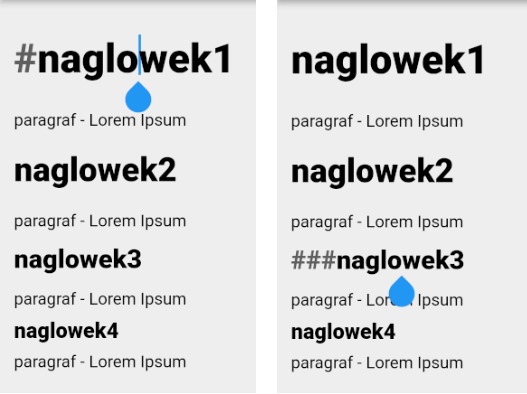
\includegraphics[height=6cm]{images/pokazywanie_naglowkow.png}
    \caption{Odkryte znaki w edytowanych nagłówkach.}
\end{figure}

\subsubsection{Ustawianie styli}

Kolejną rzeczą dostępną w aplikacji MobiNote są style. Użytkownik, chcąc poprawnie nadać style, wprowadza do tekstu symbole specjalne oznaczające konkretne style.
Odbywa się to według poniższych zasad:

\begin{itemize}
    \setlength\itemsep{2mm}

    \item za początek oznaczenia stylu uznawany jest wzór: \newline
    \verb|[dowolny znak][symbol stylu][znak niebędący białym znakiem]|
    
    \item za koniec oznaczenia stylu uznawany jest wzór: \newline
    \verb|[znak niebędący białym znakiem][symbol stylu]|
    
    \item style mogą być łączone -- wewnątrz stylu A można dodać styl B

    \item style nie mogą być krzyżowane -- jeśli zaczynamy styl B wewnątrz stylu A, to znak końca stylu B powinien nastąpić przed symbolem końca A. 
\end{itemize}

\begin{figure}[ht]
    \centering
    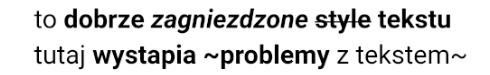
\includegraphics[width=8cm]{images/style.png}
    \caption{Zagnieżdżone style w prawidłowy i nieprawidłowy sposób}
    \vspace{3mm}
\end{figure}

\begin{figure}[ht]
    \centering
    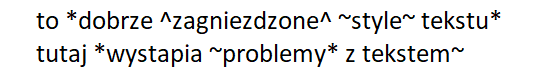
\includegraphics[width=8cm]{images/style_surowy_tekst.png}
    \caption{Surowy tekst ukazujący rozmieszczenie znaków.}
    \vspace{3mm}
\end{figure}

\subsubsection{Znaki specjalne}

Każdy dostępny styl tekstu oznaczony jest za pomocą znaków:

\begin{compactitem}
    
    \item [*] \hspace{1mm} -- pogrubienie
    \item [\^{}] \hspace{1mm} -- kursywa
    \item [\_{}] \hspace{1mm} -- podkreślenie
    \item [\~{}] \hspace{1mm} -- przekreślenie
\end{compactitem}

\subsubsection{Odkrywanie znakow specjalnych}

Edytor tekstu posiada funkcję odwijania stylu w moemncie gdy kursor znajduje się bezpośrednio w środku stylu. Odwijany jest tylko styl, którego jeden ze znaków specjalnych znajduje się najbliżej kursora. Funkcjonalność ta została wprowadzona, aby użytkownik mógł łątwiej edytować i usuwać style.
Dzięki temu może dostrzec, gdzie konkretnie znajdują się symbole danego stylu w tekście.


\begin{figure}[ht]
    \centering
    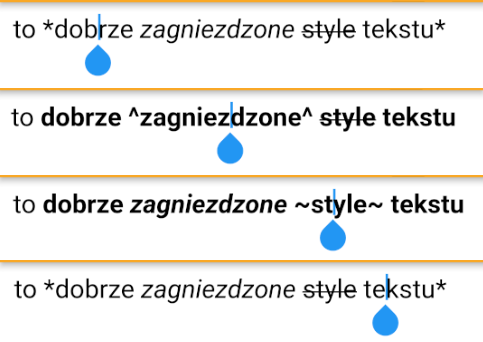
\includegraphics[width=8cm]{images/pokazywanie_znakow_specjalnych.png}
    \caption{Przykłady odkrytych znaków specjalnych.}
    \vspace{3mm}
\end{figure}

\subsubsection{Usuwanie i Edycja styli}

Aby usunąć dany styl wystarczy usunąć znaki specjalne danego stylu. Poza odkrytymi znakami reszta jest ukryta, jednak wszystkie znaki nadal występują w tekście. Edytujący może zatem kliknąć bespośrednio przed widoczny początkowy symbol lub poza tekst oznaczony danym stylem i naciskając przycisk \textbf{delete}, na klawiaturze urządzenia, usunąć dany niewidoczny symbol zakończenia stylu.

\pagebreak

\subsection{Edycja Paragrafów Widgetów}

Elementami tych paragrafów są widgety. W aktualnej wersji aplikacji dostępne są dwa widgety, które mogą być bezpośrednimi elementami paragrafów widgetów.
Są to \textbf{obrazy} i \textbf{listy}.

\subsubsection{Dodawanie}

Dodawanie paragrafów widgetów odbywa się poprzez użycie przycisków z paska narzędzi edytora notatki.

\subsubsection{Usuwanie}

Usunąć paragraf widgetów można poprzez usunięcie jego wszsytkich głównych elementów. W obecnej wersji możliwe jest posiadanie tylko jednego głównego elementu, jednak przewidziane w rozwoju aplikacji jest, aby paragrafy mogły przechowywać i używać większej ilości widgetów, w zależności od rodzajów używanych widgetów.

\subsubsection{Tryb Edycji}

Przejście do trybu edycji odbywa się poprzez interakcję z widgetem, np naciśnięcie na obraz, bądź edycja tekstu w elemencie listy.
W przypadku obrazów tryb edycji jest oznaczony poprzez dodanie obramowania do zdjęcia, jak również ikony w dolnej części obramowania służącej do zmiany rozmiaru zdjęcia.

\begin{figure}[ht]
    \centering
    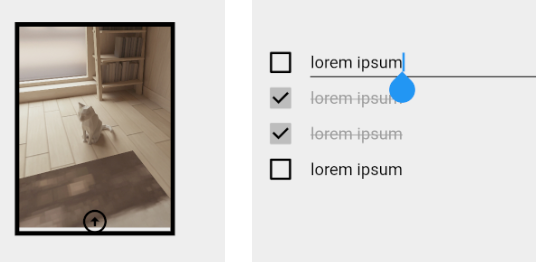
\includegraphics[width=6cm]{images/tryb_edycji.png}
    \caption{Tryb edycji przykładowych widgetów głównych.}
    \vspace{3mm}
\end{figure}

\subsubsection{Tryb zaznaczenia}

Przejście w tryb zaznaczenie odbywa się poprzez naciśnięcie i przytrzymanie konkretnych części widgetów. W przypadku obrazu jest to sam obraz, z kolei w przypadku list są to etykiety przypięte do pola tekstowego(w zależności od wyboru mogą być to: checkbox, etykiety tekstowe czy liczniki).

\begin{figure}[ht]
    \centering
    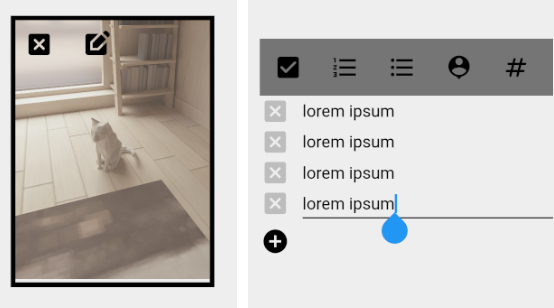
\includegraphics[width=6cm]{images/tryb_zaznaczenia.png}
    \caption{Tryb zaznaczenia przykładowych widgetów głównych.}
    \vspace{3mm}
\end{figure}


\subsection{Obrazy}

Jednym z głównych widgetów są obrazy. 

Dodawane są poprzez użycie przycisku na pasku narzędzi(sekcja: Pasek Narzędzi: Dodanie obrazu). Obraz wybierany jest z pamięci urządzenia.

\subsubsection{Edycja}

Aby zmienić rozmiar zdjęcia użytkownik musi przejść w tryb edycji poprzez kliknięcie na zdjęcie, a następnie przeciągać ikonę ze strzałką(Rysunek 3.8). Automatycznie dostosowywany będzie rozmiar obrazu.

\subsubsection{Usunięcie i zmiana}

Po wejściu w tryb zaznaczenia ukażą się dwie ikony. Ikona usunięcia obrazu oraz ikona zmiany obrazu.
Wybór pierwszej ikony skutkuje usunięciem obrazu wraz z paragrafem, natomiast drugiej -- przejściem do pamięci urządzenia w celu wyboru zdjęcia.

\subsection{Listy}

Dostępne są różne rodzaje list. Różnią sie one głównie etykietą oraz niewielkimi kwestiami, jak na przykład dostępne przekreślenie i zmiana koloru tekstu przy odznaczonej pozycji.

\subsubsection{Edycja}

Edycja list następuje poprzez interakcję użytkownika. Użytkownik może naciskać bezpośrednio na etykiety przy polu tekstowym w celu ich edycji(checkbox, licznik), jak również edytować tekst wiersza.

W przypadku niektórych typów wiersza możliwe jest jego odznaczenie. Wówczas tekst wiersza zmienia kolor na szary, a sam tekst zostaje przekreślony.

\subsubsection{Dodawanie wierszy}

Dodawanie wierszy następuje na dwa sposoby:

\begin{enumerate}
    \item W dowolnym miejscu listy poprzez dodanie znaku nowej linii.
    \item Na koniec listy poprzez kliknięcie przycisku "+" pod etykietami w trybie zaznaczenia. 
\end{enumerate}

Dodawanie wierszy poprzez znak nowej linii przenosi tekst na prawo od miejsca dodania znaku nowej linii do nowego wiersza.

\subsubsection{Usuwanie wierszy}

Usuwanie wierszy jest możliwe w trybie zaznaczania poprzez klikanie na etykiety ze znakiem "x".

\subsubsection{Zmiana typu wierszy}

Użytkownik może zmianić typ wszystkich wierszy w danej liście poprzez przejście w tryb zaznaczenia, a następnie w górym pasku nad listą(Rysunek 3.8) wybrać jedną z dostępnych opcji.

\subsubsection{Dostępne typy wiersza}

\begin{itemize}
    \item checkbox
    \item numerowane
    \item oznaczone przez symbol "\--{}"
    \item naznaczane przez symbol "*"(w nowszej wersji aplikacji spodziewane jest tworzenie etykiet przez użytkownika)
    \item licznik
\end{itemize}

Aktualnie listy są jednopoziomowe, bez możliwości zmiany wysunięcia od początku wiersza. Możliwość ta jest przewidziana na rozwój aplikacji.

\subsubsection{Licznik}

Licznik służy do odliczania rzeczy opisywanej przez tekst wiersza. Z każdym kliknięciem zwiększana jest wartość licznika(lewa część etykiety), aż do osiągnięcia celu licznika(liczba w prawej części licznika). Wraz z osiągnięciem ustalonego celu wiersz zostaje odznaczony.

Możliwa jest zmiana wartości celu licznika. W tym celu wystarczy nacisnąć na liczbę w prawej części licznika, a następnie wybrać liczbę na klawiaturze i zatwierdzić. Po zmianie następuje reset licznika.


\begin{figure}[ht]
    \centering
    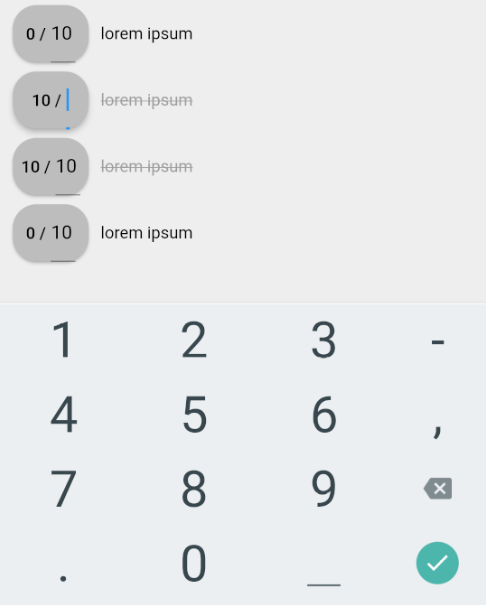
\includegraphics[width=6cm]{images/liczniki.png}
    \caption{Edycja celu jednego z liczników.}
    \vspace{3mm}
\end{figure}